%----------------------------------------------------------------------------
\chapter{Szakirodalmi áttekintés}
\label{sec:Szakirodalom}
%----------------------------------------------------------------------------
\section{Szenzorok megoldásai}
%----------------------------------------------------------------------------

A szenzorválasztás a tervezési folyamat egyik központi eleme. Meghatározza milyen technológiákkal, módszerekkel hajtjuk végre a méréseket, és ezáltal milyen kapacitású, programozású rendszert kell válasszunk. A szenzorokat érintő kutatómunka ezt a választási folyamatot segíti elő, hiszen az összes népszerű lehetőség tudatában lehet egy informált döntést hozni. ++

\subsection{Mérendő mennyiségek}

A feladatom során, a nyomatékhatároló csúszásának meghatározásához az azt megelőző és azutáni tengelyek fordulatszámának összehasonlítására van szükség. A harmadik fordulatszámmérés a felszedő tengelyen történik meg, kifejezetten az operátor informálása céljából. Egy tengely fordulatszámának mérésére több megközelítés is létezik. Lehetséges a tengely elfordulásának közvetlen mérése, akár fordulatonként egyszer történő jeladás regisztrálása, vagy a tengely kerületén érzékelhető folyamatos változás. A fordulatszám más mért mennyiségekből is származtatható, például integrálás útján gyorsulásmérésből, vagy deriválással szögelfordulásból, azonban ezeknek a pontossága nem minden esetben megfelelő, valamint a számítási igénye is magasabb az ilyen módon származtatott jeleknek \cite{Morris2016a}.

\subsection{Elmozdulás érzékelése}

Az elmozdulás mérése általában egy adott távolság, szögelfordulás tartományán belül alkalmazható, így folyamatos elfordulást mérni csak limitált fordulatszám mellett alkalmasak. A fordulatok mérésénél ezért általában a kerület mentén történő távolságbeli különbség mérése valósul meg, elmozdulás vagy pozíció érzékelésén keresztül. Erre a kerület menti geometriát (pl. fogaskerekek), egy segédlemezzel kialakított változást, vagy akár egy felhelyezett jeladó (pl. mágnes) érzékelés is mérhető.

\subsubsection{Potenciométer}

Az elmozdulás vagy pozíció érzékelésének alapvető szenzora a potenciométer, amely akár lineáris, akár elfordulás mérésére is alkalmas. 
A potenciométer működési mechanizmusa a vezetékek ellenállásán alapszik. Egy vezeték ellenállása lineárisan növekszik a hosszával, így a hosszának változása a rajta eső feszültségen keresztül mérhető. A hosszváltozás eléréséhez egy csúszka teremt kapcsolatot a vezetékkel, amelyen a vezeték végéhez képesti potenciált mérjük. A potenciál a \ref{poti} összefüggésből kapható meg, ahol $E$ a tápfeszültség, $d$ az elmozdulás, $D$ pedig a teljes elmozdulás \cite{Fraden2016a}.
\begin{equation}
	V = E \frac{d}{D}
	\label{poti}
\end{equation}
A potenciométeres szenzoroknak többféle megvalósítása is létezik. A legalapvetőbb lineáris vezeték elvén egy tekercset is lehetséges vezetékként használni, így valamivel pontosabb, nagyobb felbontású érzékelést eredményez. Léteznek potenciálmérés alapú nyomásmérő, valamint piezoelektromosságon alapuló deformáció mérésre alkalmas cellák \cite{Fraden2016a}.
Az elektromos potenciál alapú szenzorok széles felhasználásuk mellett rendelkeznek számos hátránnyal is:
\begin{itemize}
	\item Mechanikai terhelés által súrlódás
	\item Fizikai érintkezés szüksége
	\item Korlátozott sebesség
	\item Veszteségek miatti hő termelődés
	\item Szennyeződések és kopásoknak való kitettség
\end{itemize}
A fizikai kontaktus elkerülésére alkalmaznak mágneses elven működő potenciométereket. Ezeknél a szenzoroknál a csúszka egy ferromágneses bevonattal van ellátva, a vezeték alatt pedig egy mágneses réteg helyezkedik el, amelyet a csúszka vonzása összeérint a vezetékkel, így zárva az áramkört és feszültséget adva az eszközre.

\subsubsection{Kapacitív szenzorok}

A kapacitív érzékelők elmozdulás és pozíció meghatározására is alkalmasak, a későbbiekben ismertetésre kerülő mágneses alapú szenzorokkal ellentétben bármilyen anyag jelenlétét képesek érzékelni.
A kondenzátorok kapacitása fordítottan arányos a fegyverzetek közötti távolsággal, ami meglapozza a kapacitív szenzorok működését. A kapacitás változását a távolság változása vagy a fegyverzetek között található közeg változása okozhatja, amely a gyakorlatban elmozdulásmérésre alkalmas, a kapacitás változásának elektromos jellé alakításával.
A kapacitív szenzoroknak több kialakítása is alkalmazható elmozdulásmérésre, valamint egy szenzorok részeként, ahol az elmozdulást egy erő, nyomás vagy hőmérséklet változásainak dekódolására alkalmazhatják.
A monopoláris kapacitív érzékelő egy kondenzátor alkalmazására értendő, ahol két fegyverzet mozgása regisztrálódik. Az egyik fegyverzeten mérhető az elektromos jel, a másik fegyverzet azonban lehet például egy vezető felület is, mint ahogy a \ref{kapacitiv_kabel} ábrán látható szenzor kialakítása is mutatja \cite{Fraden2016a}. Ezek a szenzorok akár 40 kHz-es mérési frekvenciát is képesek produkálni, valamint nem vezető felületeken is működőképes, habár alacsonyabb pontossággal.
\begin{figure}
	\centering
	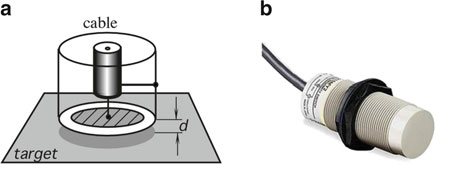
\includegraphics{figures/kapacitiv_szenzor_kabeles.png}
	\caption{Monopoláris, egylemezes kondenzátor vezető felületek távolság mérésére alkalmazva. (\textbf{a}) metszetként; (\textbf{b}) kívülről}
	\label{kapacitiv_kabel}
\end{figure}
Egy másik kialakítás a differenciál kapacitív érzékelő, amely során három fegyverzet két egyforma térrészt választ el. A középen elhelyezkedő lemez legkisebb mozgása során is megjelenik az így kialakult két kondenzátor kapacitásán, és egy változó jellel táplálva a pontos elmozdulás meghatározására is képes.
Egy kapacitív hidat látunk a \ref{kapacitiv_hid} ábrán. A szenzor két párhuzamosan elrendezett elektróda készletből állnak, konstans $d$ távolsággal közöttük, melyek közül a négy lemezből álló készlet statikus, míg a két fegyverzet elmozdulhat. A négy lemez keresztbe van kötve, így kialakítva az úgynevezett Wheatstone-híd architektúrát, melynek előnye, hogy a mérés linearitását megtartja, valamint a zajok megjelenését is minimalizálja. A párhuzamos lemezek kapacitása arányos a vele szemben lévő fegyverzetek területével, így a két kondenzátor egymáshoz képesti kisebb elmozdulását vagy elfordulását is képes detektálni. 
\begin{figure}
	\centering
	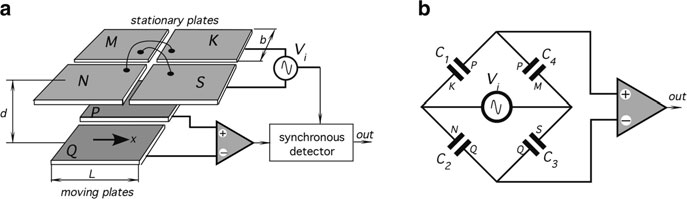
\includegraphics{figures/kapacitiv_hid.png}
	\caption{Párhuzamos lemezű kapacitív híd szenzorbeli elhelyezése (\textbf{a}) és áramköri rajz (\textbf{b})}
	\label{kapacitiv_hid}
\end{figure}

\subsubsection{Induktív szenzorok}

Induktív szenzorok azok, amelyek mágneses tereket tulajdonságait érzékelik, és így csak mágnesezhető anyagok detektálására alkalmasak. A rozsdamentes acél, alumínium, réz, műanyag, kerámia és fa anyagok áthatolhatóak a mágneses terek szempontjából, így ezekből az anyagokból készült rétegeken keresztül is érzékelhetőek a mágnesezett anyagok. Az induktív szenzorok ezáltal működnek zajos, szennyező (poros, olajos) környezetben is, valamint ezáltal az érzékelőkön a helyzetnek megfelelő anyagból készült burkolatokat lehet alkalmazni, amely veszélyesebb, korrozívabb helyzetekben is megengedi működésüket.\\
Több elv alapján és több kialakítással is érzékelhetjük a mágneses tereket.
\begin{itemize}
	\item \textbf{Elektromágneses indukció}. Két tekercs között mágneses fluxus biztosít kapcsolatot, amelyhez kell az első (primer) tekercs változó áramú gerjesztése, mely így - fázisban - megjelenik a második (szekunder) tekercsen is (önindukció elve). Ezt a kapcsolatot tudják befolyásolni különböző ferromágneses anyagok, a fluxus utakban való mozgatásuk során, ezáltal a fluxus módosításával. Ez a fluxusbeli változás mérhető feszültség változást eredményez a szekunder tekercsen. Ez adja a lineáris (és a forgó) változó differenciális transzformátor (LVDT, RVDT) szenzorok alapjait, amelyek ferromágneses anyagok lineáris- vagy forgómozgását képesek érzékelni a két tekercs közötti mágneses térben. Ennek a kialakításnak számos előnye van, például az érintkezésmentes kialakítás, elhanyagolható hiszterézis, így kevés feszültségveszteség a működés során, alacsony kitettség zajoknak és interferenciáknak, robusztus kialakítás és infinitezimális felbontás lehetősége \cite{Fraden2016a}.
	\item \textbf{Örvényáramok}. Az örvényáramok két esetben jelennek meg: amikor egy vezető elmozdul egy elektromágneses térhez képest, vagy a mágneses tér változása következtében. Az örvénylő elektronok a vezető anyagban saját elektromágneses mezőket indukálnak, amelyek az eredeti mágneses teret csökkentik. Ha erősebb a mágneses tér, vagy nagyobb a vezetőképessége az anyagnak, vagy gyorsabban változik a mágneses tér, akkor arányosan több örvényáram jön létre. Ezáltal olyan vezető anyagok elmozdulását is lehet érzékelni, amelyek nem mágnesezhetők. Az ezen elven alapuló szenzorok két tekercset alkalmaznak, az egyik referenciaként szolgál, a másik pedig érzékeli a vezetőben létrejövő örvényáramokat, a mágneses ellenállás megnövekedéséből. A két tekercs összehasonlítása során a mágneses ellenállás különbségből adódik a vezető felület távolsága. Az örvényáramok azonban egy adott vastagságú anyagban számottevőek, így a vékony filmszerű illetve bevonattal ellátott anyagok detektálására nem alkalmasak az ilyen szenzorok. Hasonló elven az örvényáramszenzorok nem csak elmozdulás, de távolság és anyagvastagság meghatározására is alkalmasak. Az érzékelő tekercsek akár 2-3 mm-es átmérőtől 25 mm-ig terjedhetnek, így nagy mérési tartomány lefedésére képesek. A nem mágneses vezetők érzékelése miatt alkalmas olyan magas hőmérsékleten való érzékelésre, ahol az anyagok elvesztik mágneses tulajdonságukat (Curie hőmérséklet felett), valamint vezető folyadékok, így folyékony fémek is érzékelhetőek az örvényáramszenzorokkal. További előnyei, hogy nincs fizikai kapcsolatra igény az detektáláshoz, így a terhelés mindig alacsony a szenzoron \cite{Fraden2016a}.
	\item \textbf{Hall-effektus}. A Hall-effektus szenzorok lényegében a mágneses terek nagyságát képesek mérni. A szenzorban egy vezető anyagból készült lemez merőlegesen áll a mágneses térre, ahogy azt a \ref{hall_effektus} ábra is szemlélteti \cite{Morris2016}. Ha a vezetőben áram folyik, az elektronokra a mágneses mező oldalirány erőt fejt ki (Lorentz-erő), ezáltal a lemezben töltésmegoszlás jön létre, amely a két szélén Hall-feszültségként mérhető \cite{Fraden2016}. A Hall érzékelős pozíciómérés során egy mágneses mezőt biztosítunk a szenzorban, amelynek a nagysága változik egy ferromágneses test jelenlétében. A szenzortól való távolság pedig, az így indukált mágneses tér módosulásából eredő feszültség változásból következik \cite{Morris2016}. 
	\begin{figure}
		\centering
		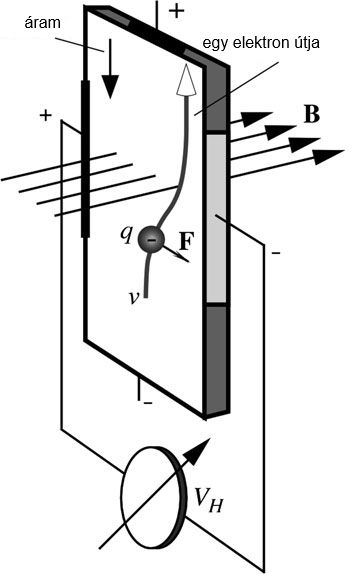
\includegraphics[width=\columnwidth/4]{figures/hall_effektus.png}
		\caption{Hall-effektus szenzor működési elve.}
		\label{hall_effektus}
	\end{figure}
\end{itemize}
Összességében a mágneses szenzorok előnye, hogy nagy felbontással és megbízhatósággal dolgoznak, valamint nincs szükségük mechanikai kapcsolatra a mérés véghezviteléhez. Azonban nagyrészt csak mágneses anyagok detektálására képesek (némelyik vezetőkön is működik), és a mérési távolságuk általában limitált.

\subsubsection{Optikai szenzorok}



\subsection{Elfordulás mérése}

\subsubsection{Helikális potenciométer}

Az elfordulást lehetséges 0-360$\degree$ között mérni egy kör kerületén, vagy akár annak egy részletén is, azonban ha 360$\degree$ fölötti mérésre van szükség egy spirális szalagot szokás alkalmazni, amelyek akár 60 fordulatot is képesek mérni \cite{Morris2016b}. +áttétel, mérési tartomány növelésére.

%----------------------------------------------------------------------------
\section{Visszajelzés lehetőségei}
%----------------------------------------------------------------------------



%----------------------------------------------------------------------------
\section{Szabályozás eszközei}
%----------------------------------------------------------------------------

\subsection{Programozási technikák}
